\documentclass[letterpaper,11pt]{article}
\usepackage{graphicx}
\usepackage{listings}
\usepackage[super]{nth}
\usepackage[hyphens]{url}
\usepackage{hyperref}
\usepackage{amsmath}
\usepackage[makeroom]{cancel}
\usepackage[table]{xcolor}
\usepackage{comment}
\usepackage[space]{grffile}
\usepackage{csvsimple}

\newcommand*{\srcPath}{../src}%

\lstset{
	basicstyle=\footnotesize,
	breaklines=true,
}

\begin{document}

\begin{titlepage}

\begin{center}

\Huge{Assignment 5}

\Large{CS 532:  Introduction to Web Science}

\Large{Spring 2018}

\Large{Chandrasekhar Reddy Muthyala}

\Large Finished on \today

\end{center}

\end{titlepage}

\newpage


% =================================
% First question
% =================================
\section*{1}

\subsection*{Question}

\begin{verbatim}
CS 432/532 Web Science
Spring 2018
http://anwala.github.io/lectures/cs532-s18/

Assignment #5
Due: 11:59pm March 7

(10 points)

1.  We know the result of the Karate Club (Zachary, 1977) split.
     Prove or disprove that the result of split could have been predicted
     by the weighted graph of social interactions.  How well does the
     mathematical model represent reality?

Generously document your answer with all supporting equations, code,
graphs, arguments, etc.

Clues: 
1. Draw original Karate club graph (two connected components) 
   after split (Week 6 lecture, slide 98).
2. Run multiple iterations of graph partioning algorithm
  (e.g., Girvan-Newman Algorithm) on experimental Karate club graph   
   until the graph splits into two connected components.
3. Compare the connected components of the experimental graph (in 2.) 
   with the original connected components of the split Karate club graph 
   (in 1.). Are they similar?

Useful sources include:

* Original paper

http://aris.ss.uci.edu/~lin/76.pdf

* Slides

http://www-personal.umich.edu/~ladamic/courses/networks/si614w06/ppt/lecture18.ppt

http://clair.si.umich.edu/si767/papers/Week03/Community/CommunityDetection.pptx

* Code and data



http://konect.uni-koblenz.de/networks/ucidata-zachary

http://vlado.fmf.uni-lj.si/pub/networks/data/ucinet/ucidata.htm#zachary

https://snap.stanford.edu/snappy/doc/reference/CommunityGirvanNewman.html

http://igraph.org/python/doc/igraph-pysrc.html#Graph.community_edge_betweenness
\end{verbatim}

\clearpage
\subsection*{Answer}

To solve this problem initially I have gone through the class slides as well as URLs given in the question and got idea how to solve this problem and started coding using R and wrote script called \textbf{KarateClub.R} shown Listing \ref{lst:rscript}, namely because using the igraph library and igraphdata, which provided the karate club dataset, was vastly easier and simpler to use with graphs.

To prove that the result of this graph split could have been predicted, I decided to use the edge betweenness algorithm provided by the igraph library, which actually used the Girvan-Newman algorithm \cite{commref}. The Girvan-Newman algorithm at each step in the graph checks if: an edge has the highest ``betweenness'' it would be removed from the graph and the modularity of the graph would then be recomputed. I decided to use the $cluster\_edge\_betweenness$ function to cluster them nicely based on their strongly or weakly connections with each other actor.

The H and A nodes, as shown in Figure \ref{fig:q1orig}, represent Mr. Hi and John A respectively. It shows how they are at the center of each of their factions. Its assumed that after running the graph through the Girvan-Newman algorithm until a certain number of groups had been made with zero connections left to the other groups, that it would match fairly well like Figure \ref{fig:q1desired}. Luckily, the igraph library automatically calculated the betweenness for me and stored it an a variable that I could access and then manually delete the edges with the highest betweenness. I then checked if the number of components, or disconnected groups, was 2. 

What I found was that my actual split was 94\% accurate with with two actors being sent to the wrong group. Actors 3 and 14, making it 2/33 were grouped wrongly with John A's officer faction as shown in Figure \ref{fig:q1outcome}. This shows that this model does represent reality quite well and only missed a single actor compared to Zachary Wayne's model prediction of 97\% accuracy \cite{zachref}.

\begin{figure}[h]
\centering
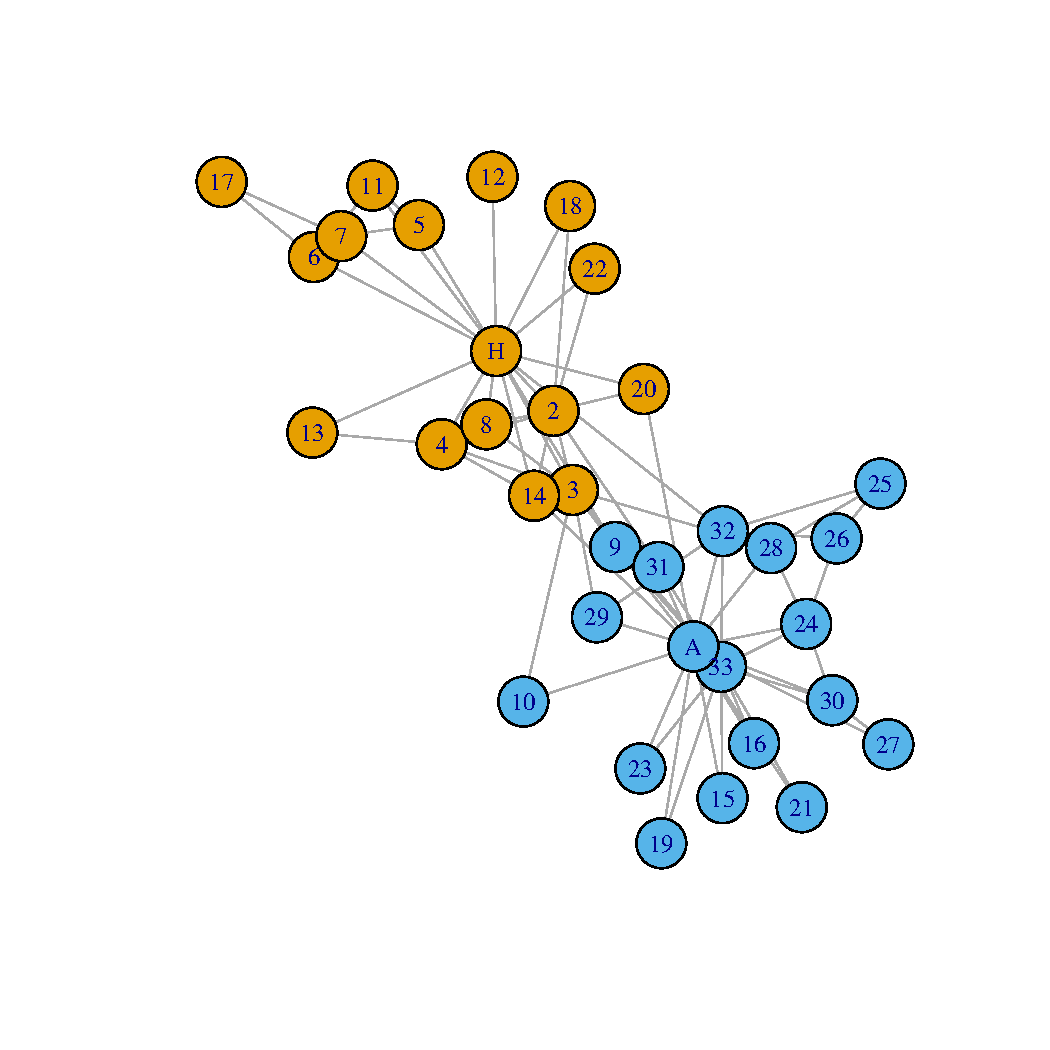
\includegraphics[scale=0.6]{intialGraph.pdf}
\caption{Original Karate Club Split}
\label{fig:q1orig}
\end{figure}

\begin{figure}[h]
\centering
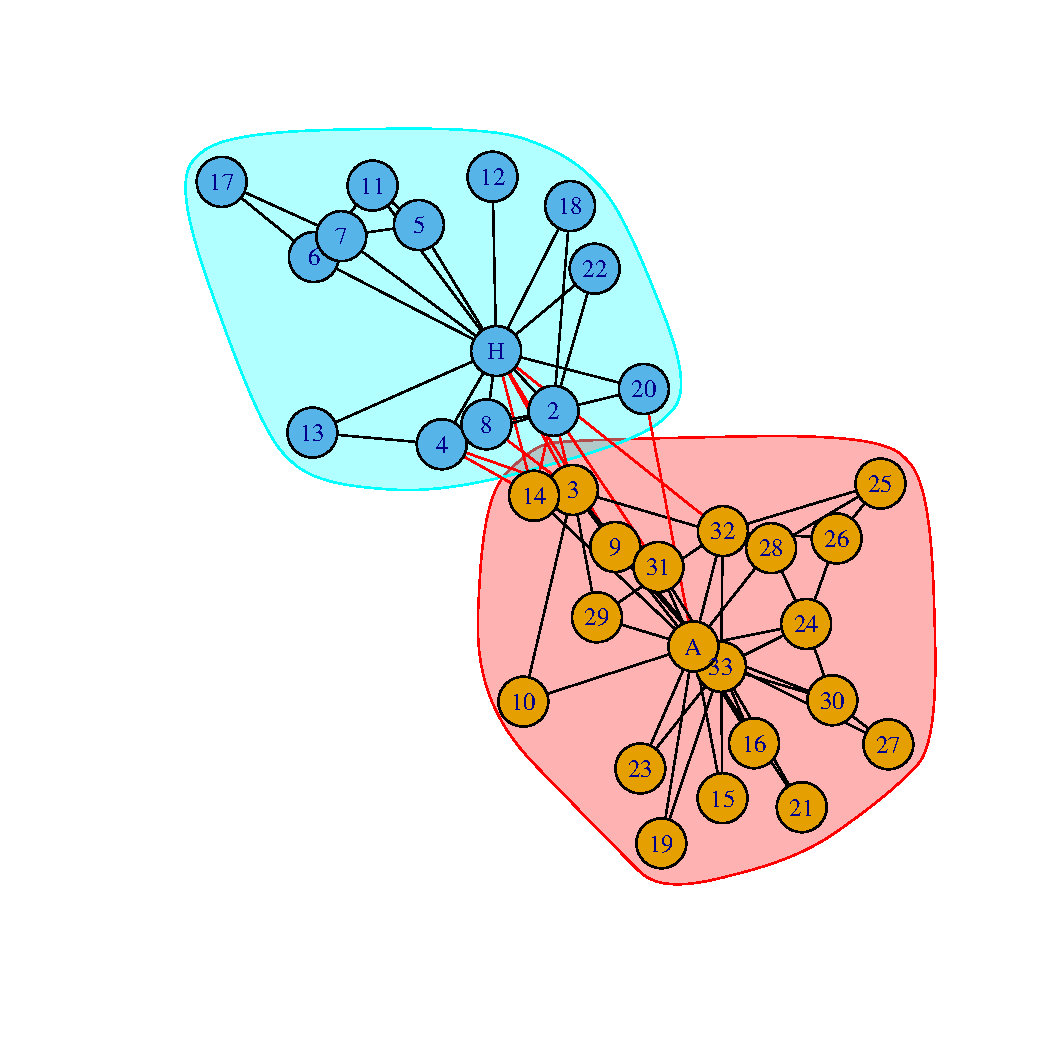
\includegraphics[scale=0.6]{CommunitiesGraph.pdf}
\caption{Desired groups when split}
\label{fig:q1desired}
\end{figure}
\clearpage
\lstinputlisting[frame=single,caption={R script for splitting groups using Girvan-Newman algorithm},label=lst:rscript,captionpos=b,numbers=left,showspaces=false,showstringspaces=false,basicstyle=\footnotesize]{KarateClub.R}

\begin{figure}[h]
\centering
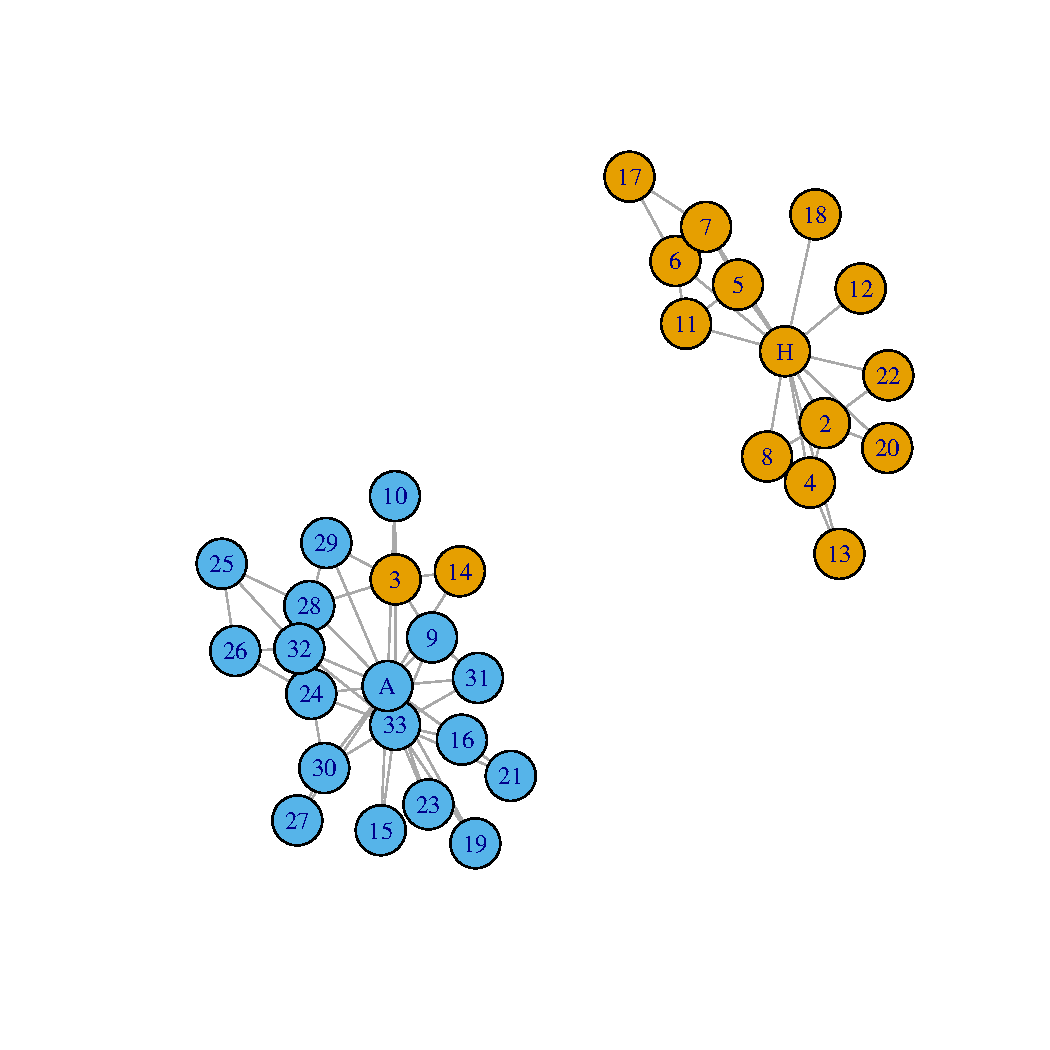
\includegraphics[scale=0.6]{predictedFinalGraph.pdf}
\caption{Actual predicted group split with Girvan-Newman from karateClub.R}
\label{fig:q1outcome}
\end{figure}

\clearpage

% =================================
% Second question
% =================================

\section*{2}

\subsection*{Question}

\begin{verbatim}
(extra credit, 3 points)

2.  We know the group split in two different groups.  Suppose the
disagreements in the group were more nuanced -- what would the clubs
look like if they split into groups of 3, 4, and 5?
\end{verbatim}

\clearpage
\subsection*{Answer}

For this question I approached it the exact same as the first question. I again used the R script as shown in Listing \ref{lst:rscript} to split the karate club into further groups. In the the script I simply changed the base case for the while loop up to 3, 4 and 5, which signified how many groups were required until it would cease deleting edges. For a 3 group split this is shown in Figure \ref{fig:split3}. For a 4 group split this is shown in Figure \ref{fig:split4}. For a 5 group split this is shown in Figure \ref{fig:split5}. I didn't attempt to verify the accuracy of these group splits as I couldn't find more information regarding a split to these degrees.
All the iterations of the 2, 3, 4, 5 split graphs are  stored in \textbf{twoGroupGraph.pdf}, \textbf{threeGroupGraph.pdf} , \textbf{fourGroupGraph.pdf} , \textbf{fiveGroupGraph.pdf} 
\begin{figure}[h]
\centering
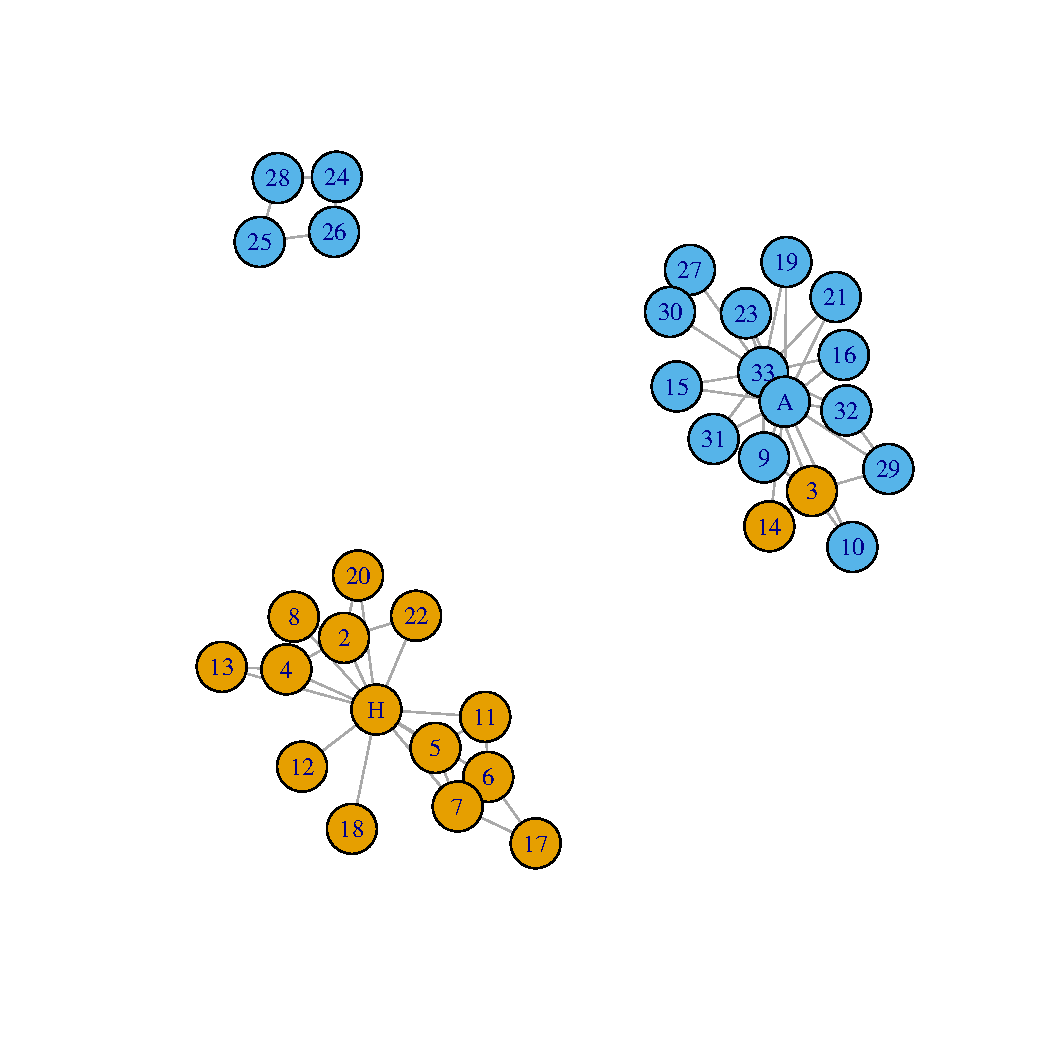
\includegraphics[scale=0.6]{TheeGroupFinalBarchart.pdf}
\caption{Group split of 3 with Girvan-Newman algorithm from karateClub.R}
\label{fig:split3}
\end{figure}

\begin{figure}[h]
\centering
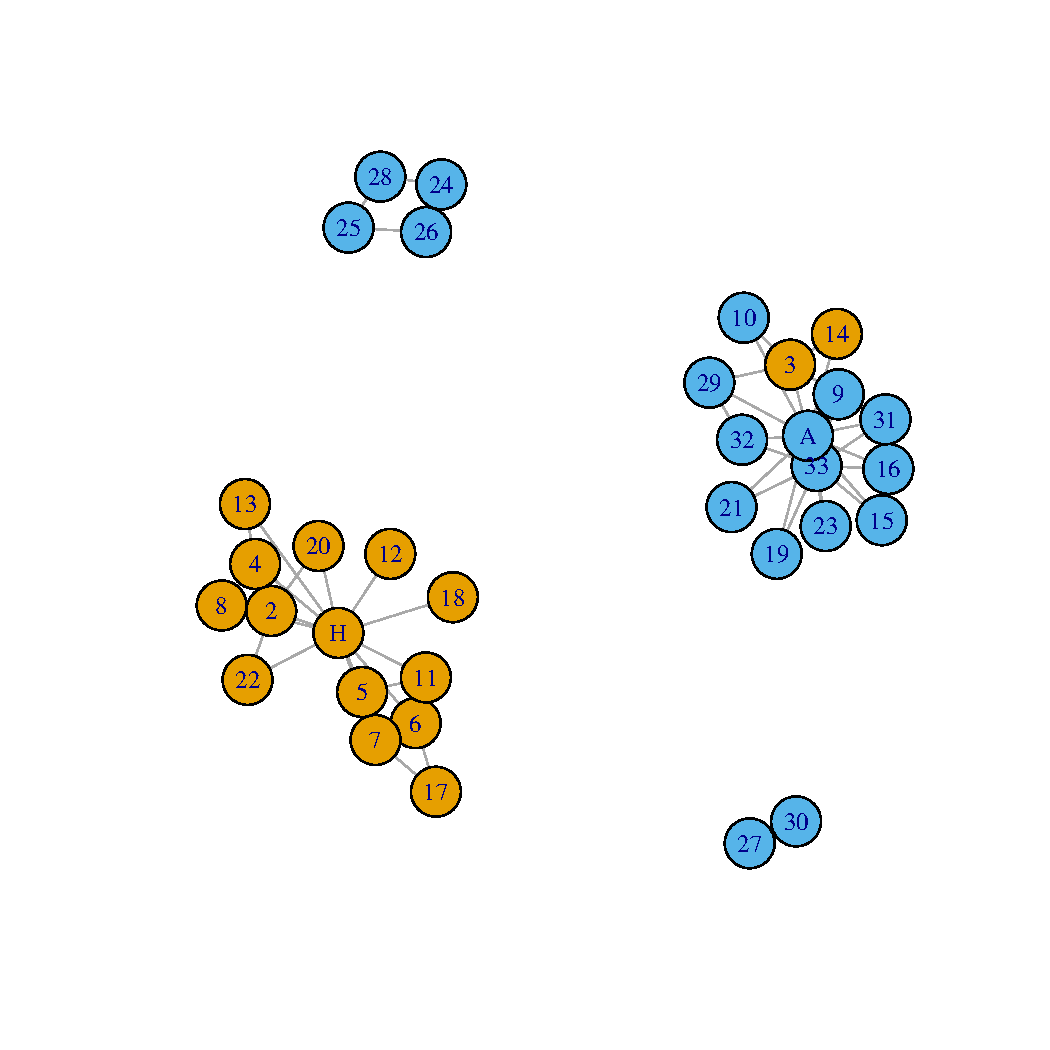
\includegraphics[scale=0.6]{FourGroupFinalBarchart.pdf}
\caption{Group split of 4 with Girvan-Newman algorithm from karateClub.R}
\label{fig:split4}
\end{figure}

\begin{figure}[h]
\centering
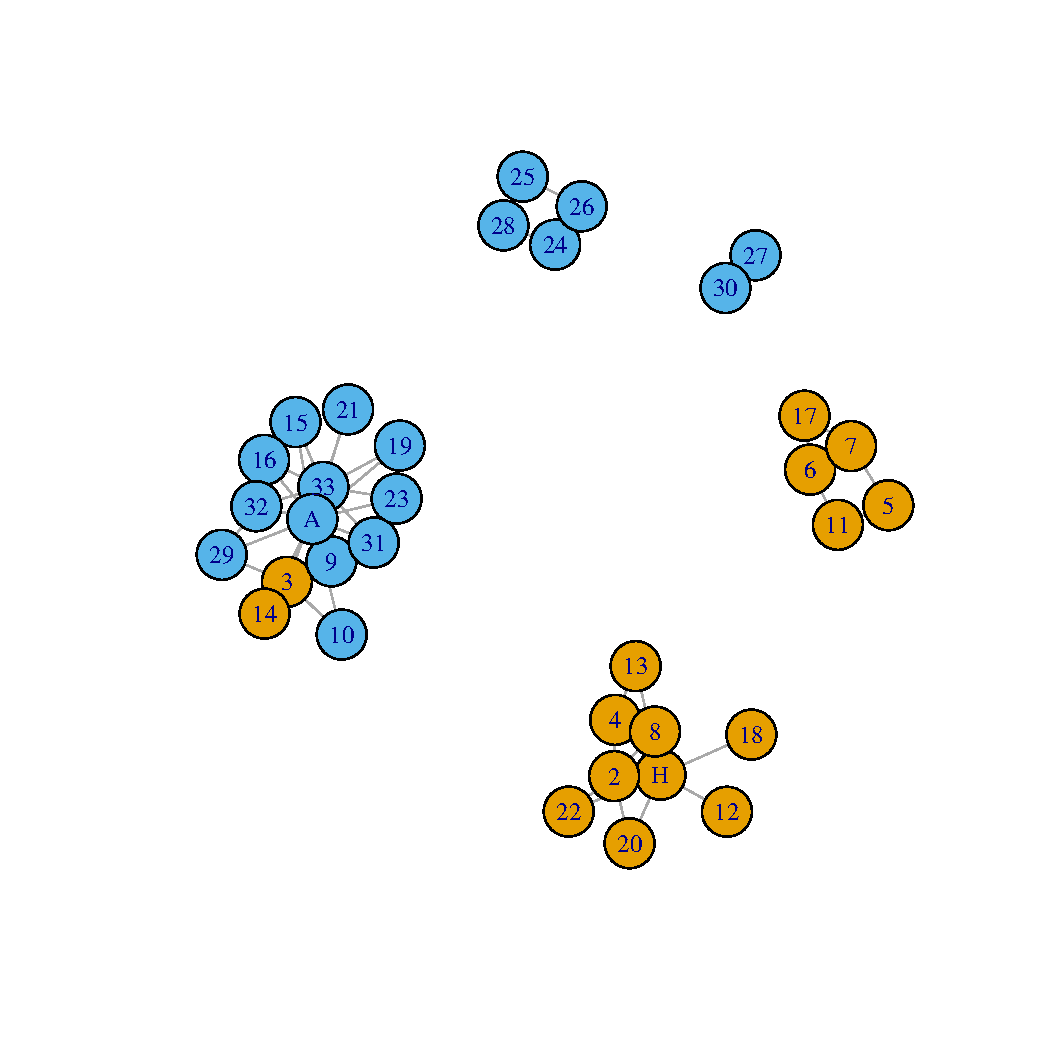
\includegraphics[scale=0.6]{FiveGroupFinalBarchart.pdf}
\caption{Group split of 5 with Girvan-Newman algorithm from karateClub.R}
\label{fig:split5}
\end{figure}



\clearpage

% =================================
% Bibliography
% =================================

\begin{thebibliography}{9}
\bibitem{igraphdataref}
Csardi, Gabor. ``Package `graphdata' '' iGraphData. Cran-R-Project, 13 July 2015. Web. 16 March 2017.\url{https://cran.r-project.org/web/packages/igraphdata/igraphdata.pdf}.
\bibitem{igraphref}
Csardi, Gabor, ``Package `igraph' '' iGraph. Cran-R-Project, 13 July 2015. Web. 16 March 2017. \url{http://igraph.org/r/doc/igraph.pdf}.
\bibitem{commref}
Rodrigues, David.``Finding Communities in networks with R and igraph'' N.p., n.d. Web. 16 March 2017. \url{http://www.sixhat.net/finding-communities-in-networks-with-r-and-igraph.html}.
\bibitem{zachref}
W. W. Zachary, An information flow model for conflict and fission in small groups, Journal of Anthropological Research 33, 452-473 (1977).
\end{thebibliography}

\end{document}